\documentclass{article}
\usepackage{neb-macros}
\usepackage{tikz}
  \usetikzlibrary{patterns}

\begin{document}

\CheapTitle{Homomorphisms}

\begin{dfn}[Ring Homomorphism]
Let $R$ and $S$ be rings. A map $\varphi : R \rightarrow S$ is called a \emph{ring homomorphism} if the following are satisfied.
\begin{itemize}
\item $\varphi(a + b) = \varphi(a) + \varphi(b)$ for all $a,b \in R$.
\item $\varphi(ab) = \varphi(a)\varphi(b)$ for all $a,b \in R$.
\end{itemize}

If $R$ and $S$ are both unital rings, we say that $\varphi$ is \emph{unital} if $\varphi(1_R) = 1_S$.
\end{dfn}

\begin{prop} \mbox{}
\begin{enumerate}
\item If $R$ is a ring, then $1 : R \rightarrow R$ given by $1(x) = x$ is a ring homomorphism. If $R$ is unital, then $1$ is unital.
\item If $\varphi : R \rightarrow S$ and $\psi : S \rightarrow T$ are ring homomorphisms, then $\psi \circ \varphi : R \rightarrow T$ is a homomorphism. If $\varphi$ and $\psi$ are unital, then $\psi \circ \varphi$ is unital.
\end{enumerate}
\end{prop}

Homomorphisms are \emph{structure-preserving maps}. The arithmetic on a ring -- the plus and times -- are a kind of structure, and homomorphisms are the maps which ``transport'' this structure to another setting. If $\varphi : R \rightarrow S$ is a ring homomorphism then in a concrete sense there is a ``shadow'' of $R$ inside $S$. If $R$ and $S$ are both unital rings, then the one element is an extra bit of structure.

\begin{prop}
Suppose $\varphi : R \rightarrow S$ is a ring homomorphism.
\begin{itemize}
\item $\varphi(0_R) = 0_S$
\item $\varphi(-a) = -\varphi(a)$ for all $a \in R$.
\item $\varphi(a-b) = \varphi(a) - \varphi(b)$ for all $a,b \in R$.
\end{itemize}
\end{prop}



\subsection*{Examples}

\begin{itemize}
\item The natural projection $\pi : \ZZ \rightarrow \ZZ/(n)$ is a unital ring homomorphism.

\item If $R$ is any ring, then there is exactly one ring homomorphism $\varphi : R \rightarrow 0$, and exactly one homomorphism $\psi : 0 \rightarrow R$. Neither of these is ever unital unless $R = 0$.

\item Let $R$ be any unital ring. Then $\varphi : R \rightarrow \MAT{2}{R}$ given by \[ \varphi(r) = \begin{bmatrix} 0 & 0 \\ -r & r \end{bmatrix} \] is a ring homomorphism. Although $R$ (and hence $\MAT{2}{R}$) is unital, $\varphi$ is \emph{not} a unital homomorphism. (Why?)
\end{itemize}



\subsection*{Images and Kernels}

\begin{dfn}[Image and Kernel]
Let $\varphi : R \rightarrow S$ be a ring homomorphism. We define subsets of $R$ and $S$ as follows.
\begin{itemize}
\item The \emph{kernel} of $\varphi$, denoted $\KER{\varphi}$, is the set \[ \KER{\varphi} = \{ r \in R \mid \varphi(r) = 0 \}. \]
\item The \emph{image} of $\varphi$, denoted $\IM{\varphi}$, is the set \[ \IM{\varphi} = \{ s \in S \mid s = \varphi(r)\ \mathrm{for\ some}\ r \in R \}. \]
\end{itemize}
\end{dfn}

\begin{prop}
If $\varphi : R \rightarrow S$ is a ring homomorphism, then $0_R \in \KER{\varphi}$ and $0_S \in \IM{\varphi}$.
\end{prop}

\begin{center}
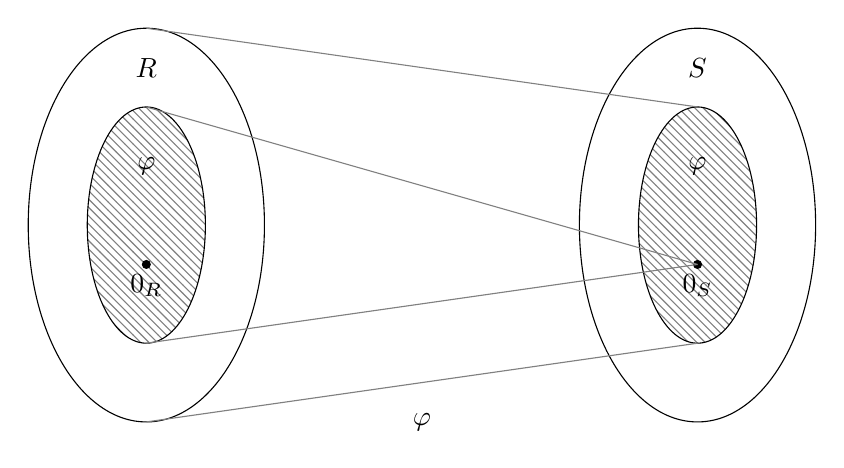
\begin{tikzpicture}[scale=0.5]
  \draw (-7,0) ellipse (3 and 5);
  \node at (-7,4) {$R$};
  \draw [pattern=north west lines, pattern color=gray] (-7,0) ellipse (1.5 and 3);
  \draw [fill] (-7,-1) circle (0.1) node [below] {$0_R$};
  \node at (-7,1.5) {$\KER{\varphi}$};

  \draw (7,0) ellipse (3 and 5);
  \node at (7,4) {$S$};
  \draw [pattern=north west lines, pattern color=gray] (7,0) ellipse (1.5 and 3);
  \draw [fill] (7,-1) circle (0.1) node [below] {$0_S$};
  \node at (7,1.5) {$\IM{\varphi}$};

  \draw [gray] (-7,3) -- (7,-1);
  \draw [gray] (-7,-3) -- (7,-1);
  \draw [gray] (-7,5) -- (7,3);
  \draw [gray] (-7,-5) -- (7,-3);

  \node at (0,-5) {$\varphi$};
\end{tikzpicture}
\end{center}

The kernel measures how badly a homomorphism fails to be injective.

\begin{prop}
A ring homomorphism $\varphi$ is injective if and only if $\KER{\varphi} = 0$.
\end{prop}


\subsection*{Characteristic}

\begin{prop}
If $R$ is a unital ring, then there is a unique unital homomorphism $\varphi : \ZZ \rightarrow R$.
\end{prop}

We can think of the image of this map as a copy of the integers in $R$, with $1 = 1_R$, $2 = 1_R + 1_R$, and so on.

\begin{dfn}[Characteristic]
Let $R$ be a unital ring and $\varphi : \ZZ \rightarrow R$ the unique unital homomorphism. If there is a positive integer $n$ such that $\varphi(n) = 0$, then there is a \emph{smallest} such integer. We call this the \emph{characteristic} of $R$, denoted $\CHAR{R}$. That is, $\CHAR{R}$ is the smallest positive natural number such that \[\underbrace{1_R + 1_R + \cdots + 1_R}_{n\ \mathrm{times}} = 0_R.\] If no such $n$ exists, we say that $\CHAR{R} = 0$.
\end{dfn}

\end{document}
